\documentclass[aspectratio=43]{beamer}

\usepackage[T2A]{fontenc}
\usepackage[utf8]{inputenc}
\usepackage[english,russian]{babel}
\usepackage{graphicx}
\usepackage{booktabs}
\usepackage{amsmath,amssymb}
\usepackage{multirow}
\usepackage{bm}

% ---- Тема: стандарт кафедры, чтобы не выделяться ----
%\usetheme{Boadilla}
\usecolortheme{beaver}
\usefonttheme[onlymath]{serif}
\setbeamertemplate{navigation symbols}{}
\setbeamertemplate{footline}[page number]
\setbeamertemplate{blocks}[rounded=true,shadow=true]
\setbeamersize{text margin left=0.5cm,text margin right=0.5cm}
\setbeamerfont{author}{size=\normalsize}
\setbeamerfont{institute}{size=\normalsize}
\setbeamerfont{date}{size=\normalsize}
\setbeamertemplate{enumerate item}{\insertenumlabel)}
\setbeamertemplate{enumerate subitem}{\insertenumlabel)}
\setbeamertemplate{enumerate subsubitem}{\insertenumlabel)}

% ---- Номер кадра в нижнем колонтитуле ----
\setbeamertemplate{footline}{%
  \leavevmode%
  \hbox{%
  \begin{beamercolorbox}[wd=.33\paperwidth,ht=2.4ex,dp=1.1ex,leftskip=.3em,rightskip=.3em]{author in head/foot}%
    \usebeamerfont{author in head/foot}\insertshortauthor%
  \end{beamercolorbox}%
  \begin{beamercolorbox}[wd=.50\paperwidth,ht=2.4ex,dp=1.1ex,center]{title in head/foot}%
    \usebeamerfont{title in head/foot}\insertshorttitle%
  \end{beamercolorbox}%
  \begin{beamercolorbox}[wd=.17\paperwidth,ht=2.4ex,dp=1.1ex,right,rightskip=.5em]{date in head/foot}%
    \usebeamerfont{date in head/foot}\insertframenumber\,/\,\inserttotalframenumber%
  \end{beamercolorbox}}%
  \vskip0pt%
}

% ---- Теоремоподобные окружения ----
\setbeamertemplate{theorems}[numbered]
\theoremstyle{definition}
\newtheorem{defn}{Определение}
\newtheorem{prop}{Утверждение}

\DeclareMathOperator*{\argmin}{arg\,min}

% ---- Компактные отступы вокруг выключных формул (плотные слайды) ----
\setlength{\abovedisplayskip}{4pt}
\setlength{\belowdisplayskip}{4pt}
\setlength{\abovedisplayshortskip}{2pt}
\setlength{\belowdisplayshortskip}{2pt}
\setlength{\emergencystretch}{2em}  % поглощает микропереполнения строк

\title[Флоу Матчинг для трансляции КТ]{Флоу Матчинг в задачах трансляции\\компьютерной томографии}
\author[Крейнин М.\,В.]{Крейнин Матвей Вадимович\texorpdfstring{\\[4pt]{\small Научный руководитель: к.ф.-м.н. А.\,В.\,Грабовой}}{}}
\institute[МФТИ]{%
  Московский физико-технический институт\\
  Физтех-школа прикладной математики и информатики\\
  Кафедра интеллектуального анализа данных ВЦ РАН\\[2pt]
  {\small 09.04.01 --- Информатика и вычислительная техника}}
\date{Москва, 2026}

% ====================================================================
\begin{document}

% ---- 1. Титул --------------------------------------------------------
\begin{frame}[plain]
  \titlepage
\end{frame}

% ---- 2. Мотивация ----------------------------------------------------
\begin{frame}{Мотивация}

\begin{block}{Цель}
Метод и архитектура нейросети для быстрой \textbf{двунаправленной} трансляции между нативными и контрастными КТ-сериями.
\end{block}

\begin{alertblock}{Проблема}
Диагностика требует обе фазы, но второе сканирование --- лучевая нагрузка; публичные датасеты содержат лишь одну фазу. Диффузионные модели требуют сотни шагов; специализированные методы работают только в одну сторону.
\end{alertblock}

\begin{exampleblock}{Предлагаемое решение}
Фреймворк \textbf{Medical Flow Matching (MFM)} с архитектурой \textbf{TimeResNet}: инъекция времени в каждый блок и свёрточный self-attention в боттлнеке.
\end{exampleblock}

\end{frame}

% ---- 3. Постановка задачи и CFM -------------------------------------
\begin{frame}{Постановка задачи и Flow Matching}
\footnotesize

\begin{defn}[Пространство и поток]
$\mathcal{X}=[-1,1]^{H\times W}$; $\pi_N,\pi_C$ --- распределения нативных и контрастных серий; пары $(\mathbf{x}_N,\mathbf{x}_C)\sim\gamma\in\Pi(\pi_N,\pi_C)$. Поле $f_\theta$ задаёт поток: $\;d\mathbf{x}_t/dt=f_\theta(\mathbf{x}_t,t)$.
\end{defn}

\vspace{-0.12cm}
\begin{block}{Релаксация и симуляционно-свободная потеря}
Интерполянт $\mathbf{x}_t=(1-t)\mathbf{x}_0+t\mathbf{x}_1$, скорость $\mathbf{v}^*=\mathbf{x}_1-\mathbf{x}_0$:
\[
  \mathcal{L}_{\mathrm{CFM}}(\theta)=\mathbb{E}_{t\sim\mathcal{U}[0,1],\,(\mathbf{x}_0,\mathbf{x}_1)\sim\gamma}\bigl[\lVert f_\theta(\mathbf{x}_t,t)-\mathbf{v}^*\rVert_2^2\bigr].
\]
Обучение симуляционно-свободно: на каждом шаге --- $\ell_2$-регрессия скорости без интегрирования ОДУ.
\end{block}

\vspace{-0.12cm}
\begin{prop}[Двунаправленность]
Для $\theta^*=\argmin_\theta\mathcal{L}_{\mathrm{CFM}}$ одна сеть реализует оба отображения: $\hat{\mathbf{x}}_C=\mathbf{x}+\int_0^1 f_{\theta^*}\,dt$, $\;\hat{\mathbf{x}}_N=\mathbf{x}+\int_1^0 f_{\theta^*}\,dt$.
\end{prop}

\end{frame}

% ---- 4. Схема метода -------------------------------------------------
\begin{frame}{Схема метода MFM}
\centering
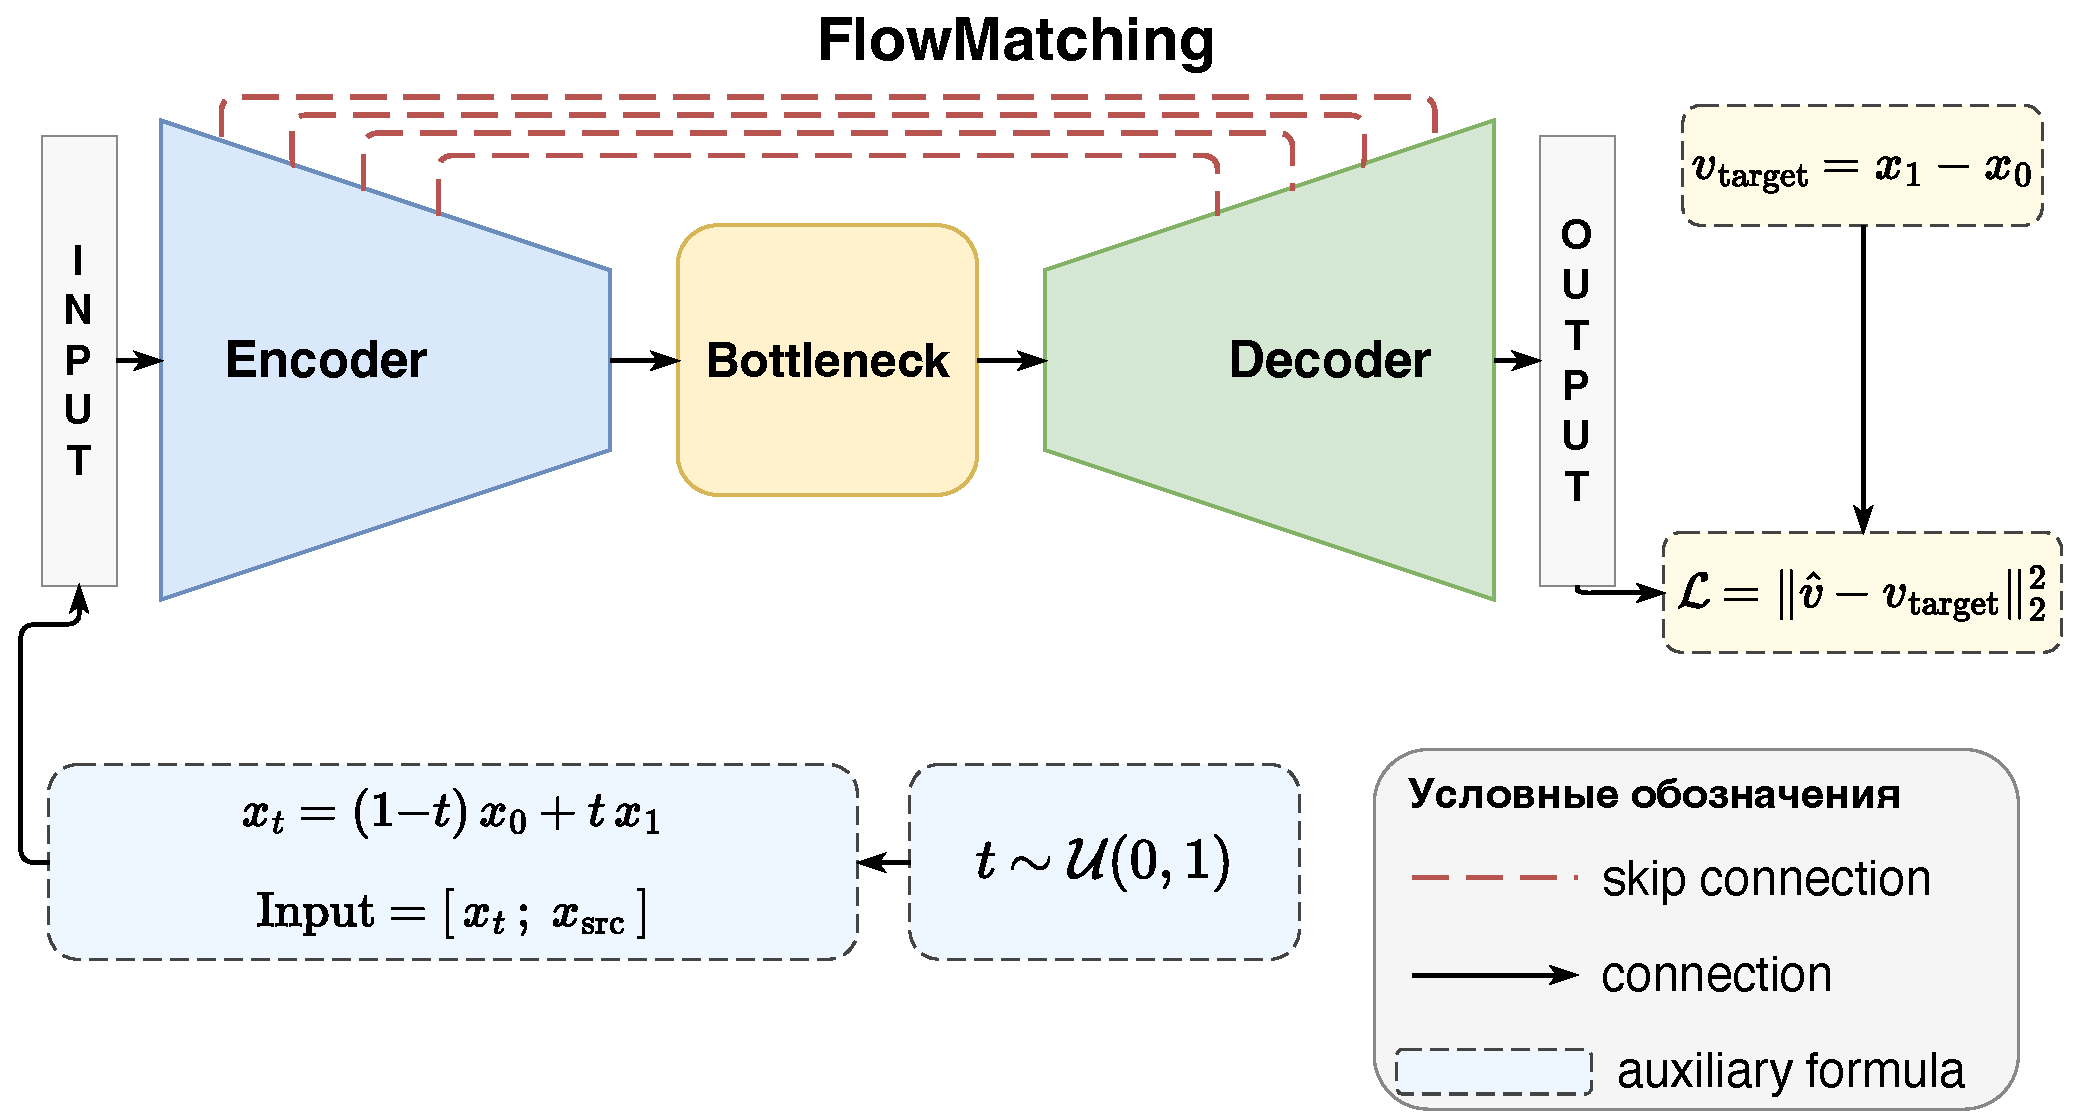
\includegraphics[width=0.93\linewidth]{images/flow.pdf}

\vspace{0.2cm}
{\small Сверху --- линейная интерполяция при разных $t$; снизу --- сеть аппроксимирует \emph{постоянную} скорость $\mathbf{x}_C-\mathbf{x}_N$. Инференс --- один шаг интегрирования ОДУ.}
\end{frame}

% ---- 5. TimeResNet: обзор -------------------------------------------
\begin{frame}{Архитектура TimeResNet}
\centering
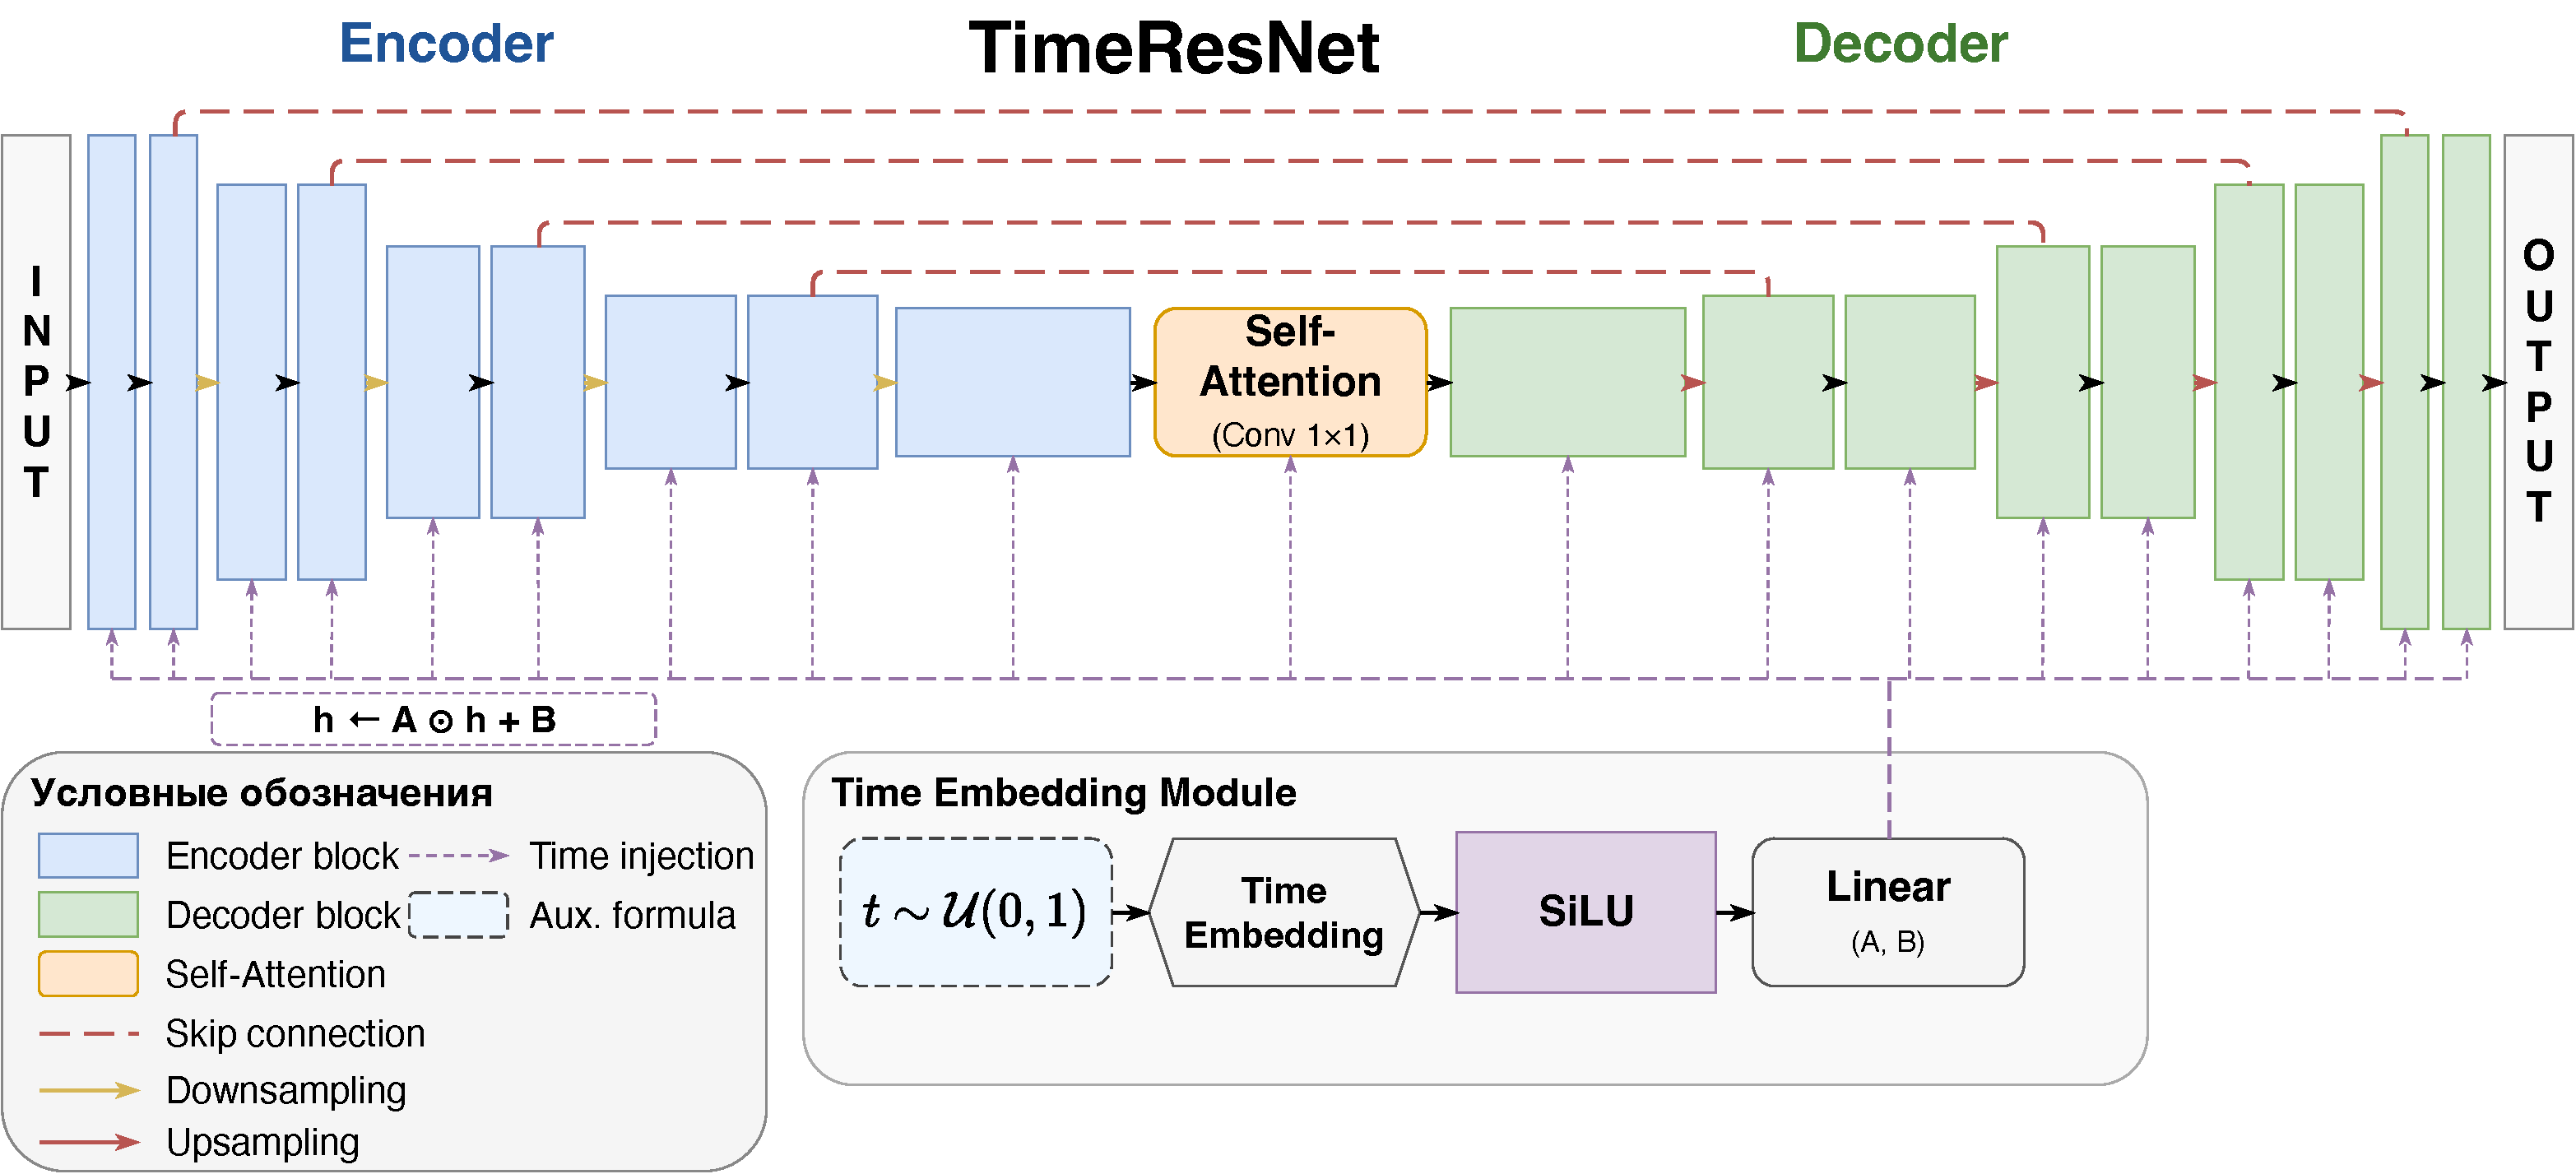
\includegraphics[width=0.80\linewidth]{images/timeresnet.pdf}

\vspace{0.15cm}
{\small U-Net encoder--decoder с двумя модификациями для флоу матчинга:
\begin{enumerate}\setlength{\itemsep}{1pt}
    \item \textbf{Поблочная инъекция времени} --- аффинная модуляция в \emph{каждом} ResNet-блоке.
    \item \textbf{Self-attention в боттлнеке} на самом грубом разрешении.
\end{enumerate}}
\end{frame}

% ---- 7. Инъекция времени + свойство ---------------------------------
\begin{frame}{Поблочная инъекция времени}
\footnotesize

\begin{columns}[c]
\begin{column}{0.40\textwidth}
\centering
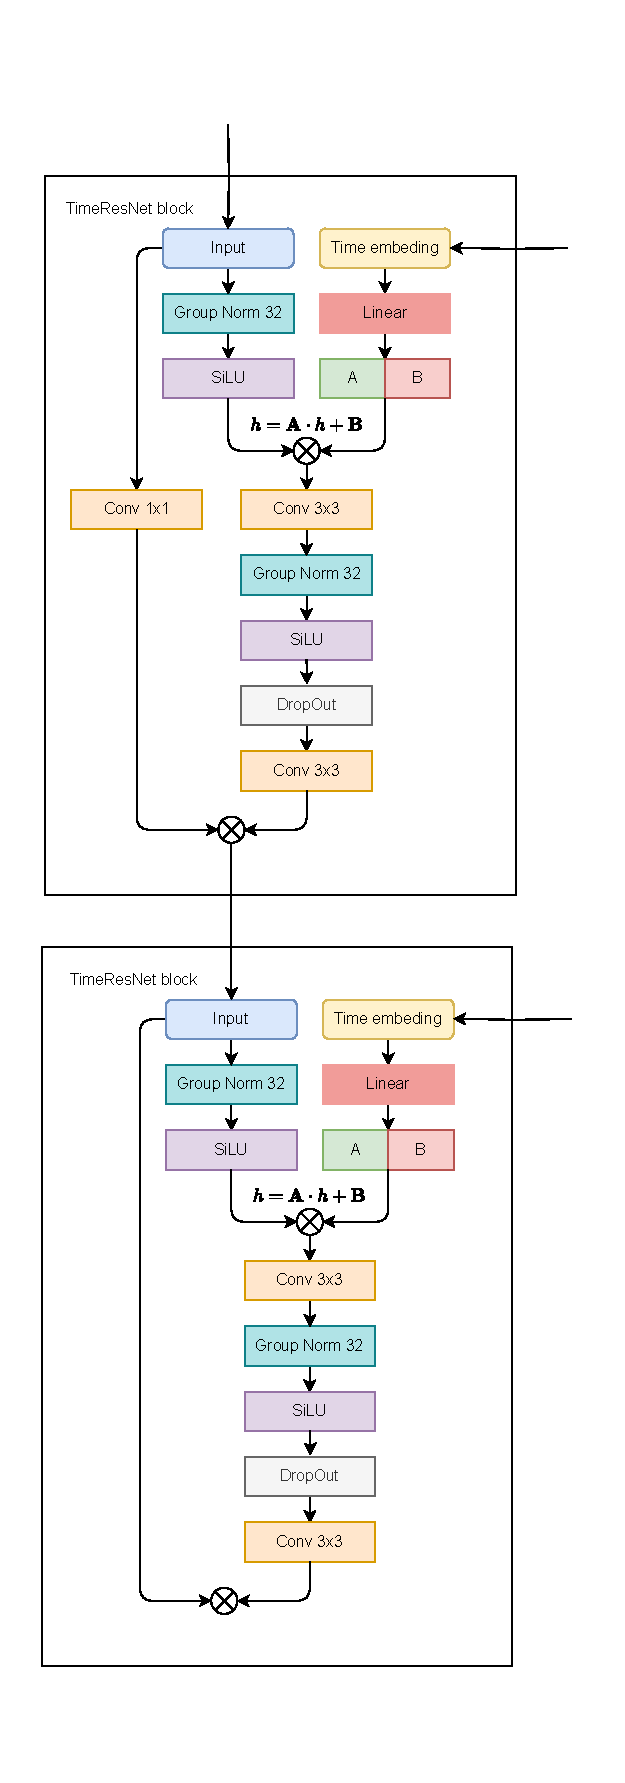
\includegraphics[trim={0 422 0 30},clip,width=\linewidth,height=0.70\textheight,keepaspectratio]{images/Embeding.pdf}
\end{column}
\begin{column}{0.60\textwidth}

\begin{defn}[Time injection]
В блоке $l=1,\dots,L$:
\[
  \mathcal{M}_l(\mathbf{h};t)=\mathbf{A}_l(t)\odot\mathbf{h}+\mathbf{B}_l(t),
\]
\[
  (\mathbf{A}_l,\mathbf{B}_l)=W_l\cdot\mathrm{MLP}\bigl(\gamma(t)\bigr),
\]
$\gamma$ --- синусоидальное кодирование, $W_l$ --- проекция блока~$l$.
\end{defn}

\begin{prop}[Сохранение временного сигнала]
\[
  \frac{\partial\mathcal{L}}{\partial t}=\sum_{l=1}^{L}\frac{\partial\mathcal{L}}{\partial\mathbf{h}_l}\cdot\frac{\partial\mathcal{M}_l}{\partial t}\neq0,\;\;\frac{\partial\mathcal{M}_l}{\partial t}\neq0\;\forall l.
\]
Сигнал не затухает по глубине (в отличие от конкатенации только со входом).
\end{prop}

\end{column}
\end{columns}

\end{frame}

% ---- 8. Self-attention + свойство -----------------------------------
\begin{frame}{Self-attention в боттлнеке}
\small

\begin{columns}[c]
\begin{column}{0.46\textwidth}
\centering
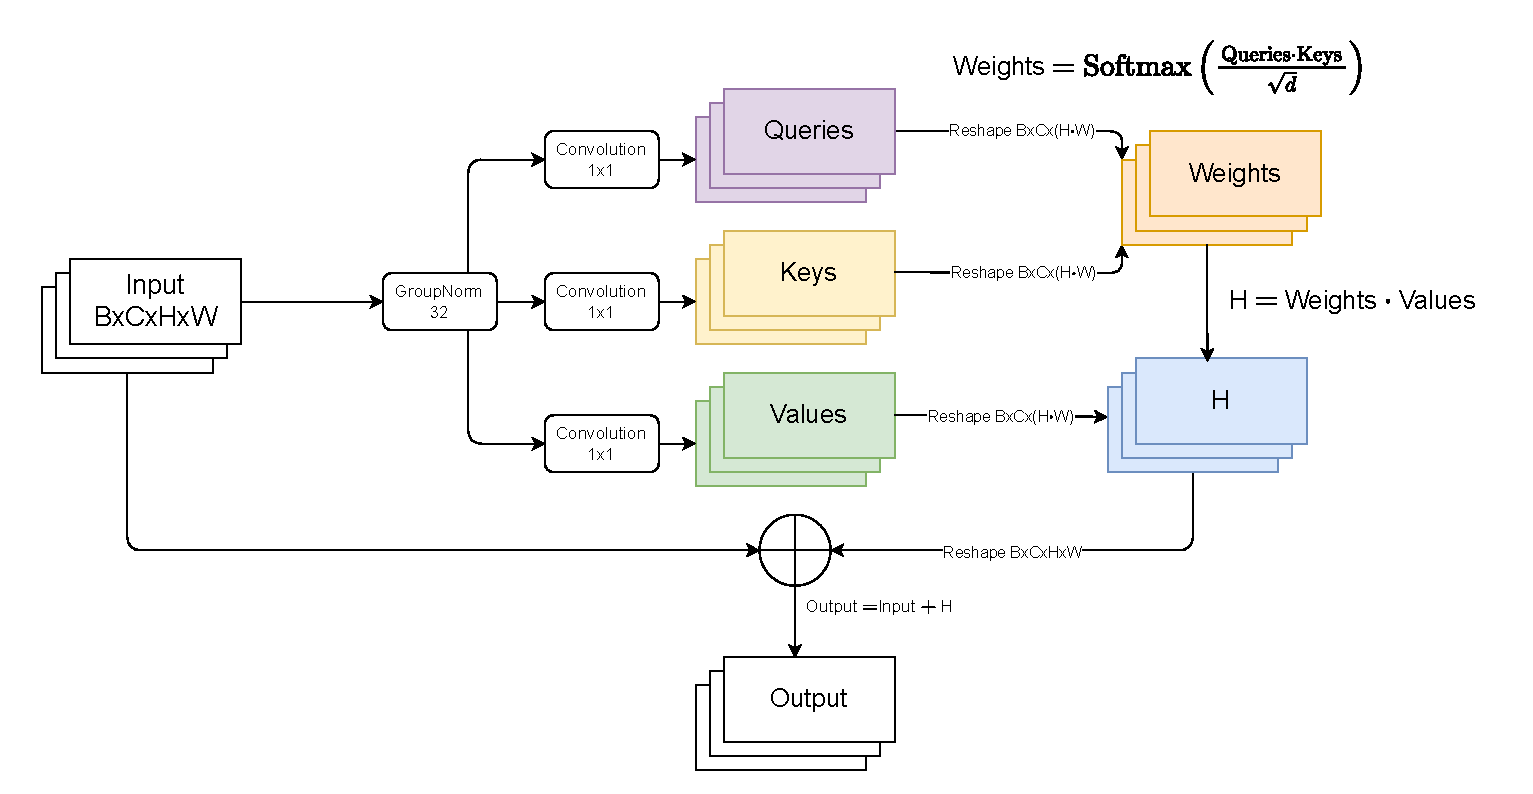
\includegraphics[width=\linewidth]{images/self_attention.pdf}
\end{column}
\begin{column}{0.54\textwidth}

\begin{defn}[Self-attention]
$Q,K,V$ --- свёртки $1{\times}1$ от входа $\mathbf{Z}\in\mathbb{R}^{C\times H'\times W'}$, $N=H'\!\cdot\!W'$:
\[
  \mathrm{Attn}(\mathbf{Z})=\mathbf{Z}+V\cdot\mathrm{softmax}\!\Bigl(\tfrac{Q^\top K}{\sqrt{C}}\Bigr).
\]
\end{defn}

\begin{prop}[Сложность в боттлнеке]
\[
  \frac{\mathcal{O}(N_{\mathrm{bottle}}^2 C)}{\mathcal{O}((HW)^2 C)}=\frac{1}{4^{2k}},\quad N_{\mathrm{bottle}}=\frac{HW}{4^{k}}.
\]
При $k=4$ --- в $\approx65\,000$ раз меньше операций, но захватывает \emph{дальние} зависимости (в отличие от оконного Swin).
\end{prop}

\end{column}
\end{columns}

\end{frame}

% ---- 9. Эксперимент C->N --------------------------------------------
\begin{frame}{Основные результаты: C\,$\to$\,N}
\footnotesize

\textbf{Данные}: 120 абдоминальных КТ (52\,561 срез), разбиение \textbf{по пациентам} 80/20/20, регистрация ANTs SyN, HU\,$[-1000,1000]\!\to\![-1,1]$.\;
\textbf{Обучение}: Adam, lr \,$= 2{\cdot}10^{-5}$, 30 эпох, 1$\times$ RTX 3090.

\vspace{-0.05cm}
\begin{table}
\centering
\renewcommand{\arraystretch}{1.05}
\resizebox{\linewidth}{!}{%
\begin{tabular}{llccccc}
\toprule
\textbf{Метод} & \textbf{Модель} & MAE$\downarrow$ & SSIM$\uparrow$ & PSNR$\uparrow$ & Time, с & Params, M \\
\midrule
\multirow{2}{*}{Регрессия}
  & SegResNet  & $6.33{\pm}1.03$ & $.982{\pm}.007$ & $38.46{\pm}1.70$ & 0.055 & 214.1 \\
  & UMambaBot  & $6.37{\pm}1.01$ & $.982{\pm}.007$ & $38.30{\pm}1.64$ & 0.075 & 141.6 \\
\midrule
Диффузия & DDPM   & $18.20{\pm}1.39$ & $.934{\pm}.008$ & $30.05{\pm}1.48$ & 44.2 & 124.7 \\
SOTA     & SMILE  & $30.22{\pm}4.95$ & $.887{\pm}.026$ & $26.70{\pm}1.33$ & 9.03 & 1066 \\
\midrule
\multirow{2}{*}{Flow Match.}
  & SegResNet           & $7.23{\pm}1.07$ & $.979{\pm}.007$ & $38.45{\pm}1.65$ & 0.065 & 214.1 \\
  & \textbf{TimeResNet} & $\mathbf{4.25{\pm}1.09}$ & $\mathbf{.994{\pm}.007}$ & $\mathbf{42.19{\pm}1.67}$ & 0.125 & 124.7 \\
\bottomrule
\end{tabular}}
\end{table}

\vspace{-0.05cm}
\centering
$\dfrac{\mathrm{MAE}_{\mathrm{SMILE}}}{\mathrm{MAE}_{\mathrm{TimeResNet}}}\approx7.1,\qquad
\dfrac{T_{\mathrm{DDPM}}}{T_{\mathrm{TimeResNet}}}\approx354.$

\flushleft\vspace{0.05cm}
{\scriptsize Разбиение по пациентам исключает утечку.}

\end{frame}

% ---- 10. N->C и органы ----------------------------------------------
\begin{frame}{Двунаправленность: N\,$\to$\,C}
\footnotesize

\begin{prop}[Единые веса для обоих направлений]
$f_{\theta^*}=\argmin_f\bigl[\mathcal{L}_{\mathrm{CFM}}^{N\to C}(f)+\mathcal{L}_{\mathrm{CFM}}^{C\to N}(f)\bigr]$ при симметричной выборке пар. Разница одно-/двунаправленного варианта --- 0.03\,HU (в пределах шума обучения). На аорте MFM точнее SMILE в \textbf{15$\times$}.
\end{prop}

\vspace{0.15cm}
\begin{columns}[T]
\begin{column}{0.55\textwidth}
\centering
{\scriptsize\textbf{Нативное $\to$ контрастное}}\\[0.1cm]
\renewcommand{\arraystretch}{1.05}
\resizebox{\linewidth}{!}{%
\begin{tabular}{lccc}
\toprule
\textbf{Модель} & MAE$\downarrow$ & SSIM$\uparrow$ & PSNR$\uparrow$ \\
\midrule
SMILE               & $21.70{\pm}4.26$ & $.903{\pm}.019$ & $29.28{\pm}1.53$ \\
SegResNet           & $6.82{\pm}0.82$  & $.983{\pm}.004$ & $37.82{\pm}1.46$ \\
SwinUNETR           & $7.36{\pm}0.78$  & $.982{\pm}.004$ & $37.52{\pm}1.32$ \\
\textbf{TimeResNet} & $\mathbf{4.57{\pm}0.87}$ & $\mathbf{.996{\pm}.004}$ & $\mathbf{41.52{\pm}1.53}$ \\
\bottomrule
\end{tabular}}
\end{column}
\begin{column}{0.45\textwidth}
\centering
{\scriptsize\textbf{MAE по органам (HU)}}\\[0.1cm]
\renewcommand{\arraystretch}{1.05}
\resizebox{\linewidth}{!}{%
\begin{tabular}{lcccc}
\toprule
\textbf{Метод} & Аорта & Почки & Печень & Подж. \\
\midrule
\multicolumn{5}{l}{\textit{C\,$\to$\,N}} \\
SegResNet (reg.) & $23.7$ & $21.8$ & $13.1$ & $17.6$ \\
SMILE & $168.5$ & $96.5$ & $97.1$ & $92.2$ \\
\textbf{MFM} & $\mathbf{16.9}$ & $\mathbf{16.4}$ & $\mathbf{9.8}$ & $\mathbf{12.7}$ \\
\midrule
\multicolumn{5}{l}{\textit{N\,$\to$\,C}} \\
SMILE & $295.8$ & $177.9$ & $63.0$ & $121.5$ \\
\textbf{MFM} & $\mathbf{20.1}$ & $\mathbf{24.3}$ & $\mathbf{12.8}$ & $\mathbf{15.4}$ \\
\bottomrule
\end{tabular}}
\end{column}
\end{columns}

\end{frame}

% ---- 11. LPIPS, согласованность, DDIM -------------------------------
\begin{frame}{Перцептивное качество и согласованность}
\footnotesize

\begin{columns}[T]
\begin{column}{0.50\textwidth}
\centering
{\scriptsize\textbf{TotalSeg-LPIPS (C\,$\to$\,N)}}\\[0.1cm]
\renewcommand{\arraystretch}{1.1}
\resizebox{\linewidth}{!}{%
\begin{tabular}{lcc}
\toprule
\textbf{Метод} & 2D$\downarrow$ & 3D$\downarrow$ \\
\midrule
SegResNet (reg.)   & $.158{\pm}.051$ & $.012{\pm}.005$ \\
SMILE              & $.704{\pm}.144$ & $.096{\pm}.044$ \\
\textbf{MFM}       & $\mathbf{.138{\pm}.053}$ & $\mathbf{.007{\pm}.004}$ \\
\bottomrule
\end{tabular}}
\end{column}
\begin{column}{0.50\textwidth}
\centering
{\scriptsize\textbf{SSIM по проекциям}}\\[0.1cm]
\renewcommand{\arraystretch}{1.1}
\resizebox{\linewidth}{!}{%
\begin{tabular}{lcccc}
\toprule
\textbf{Метод} & Акс. & Кор. & Саг. & $\Delta\downarrow$ \\
\midrule
SegResNet (reg.) & $.974$ & $.973$ & $.974$ & $.0003$ \\
SMILE            & $.852$ & $.848$ & $.847$ & $.0047$ \\
\textbf{MFM}     & $\mathbf{.984}$ & $\mathbf{.985}$ & $\mathbf{.983}$ & $\mathbf{.0001}$ \\
\bottomrule
\end{tabular}}
\end{column}
\end{columns}

\vspace{0.25cm}
\centering
{\scriptsize\textbf{Сравнение с ускоренным сэмплером диффузии (C\,$\to$\,N)}}\\[0.1cm]
\renewcommand{\arraystretch}{1.1}
\resizebox{0.9\linewidth}{!}{%
\begin{tabular}{lrcccc}
\toprule
\textbf{Метод} & Шагов & MAE$\downarrow$ & SSIM$\uparrow$ & Время, с & Замедление \\
\midrule
DDPM (полный) & $1000$ & $18.20{\pm}1.39$ & $0.934$ & $44.20$ & $354\times$ \\
DDIM-50       & $50$   & $21.07{\pm}1.61$ & $0.815$ & $5.03$  & $40\times$ \\
\textbf{MFM (Эйлер-1)} & $\mathbf{1}$ & $\mathbf{4.25{\pm}1.09}$ & $\mathbf{0.994}$ & $\mathbf{0.125}$ & $1\times$ \\
\bottomrule
\end{tabular}}

\vspace{0.1cm}
{\scriptsize $\Delta$SSIM $=0.0001$ и 3D-LPIPS $=0.007$ $\Rightarrow$ межосевая согласованность, несмотря на 2D-обработку.}

\end{frame}

% ---- 12. Визуал, ablation, downstream -------------------------------
\begin{frame}{Вклад компонент и downstream-сегментация}

\begin{columns}[c]
\begin{column}{0.56\textwidth}
\centering
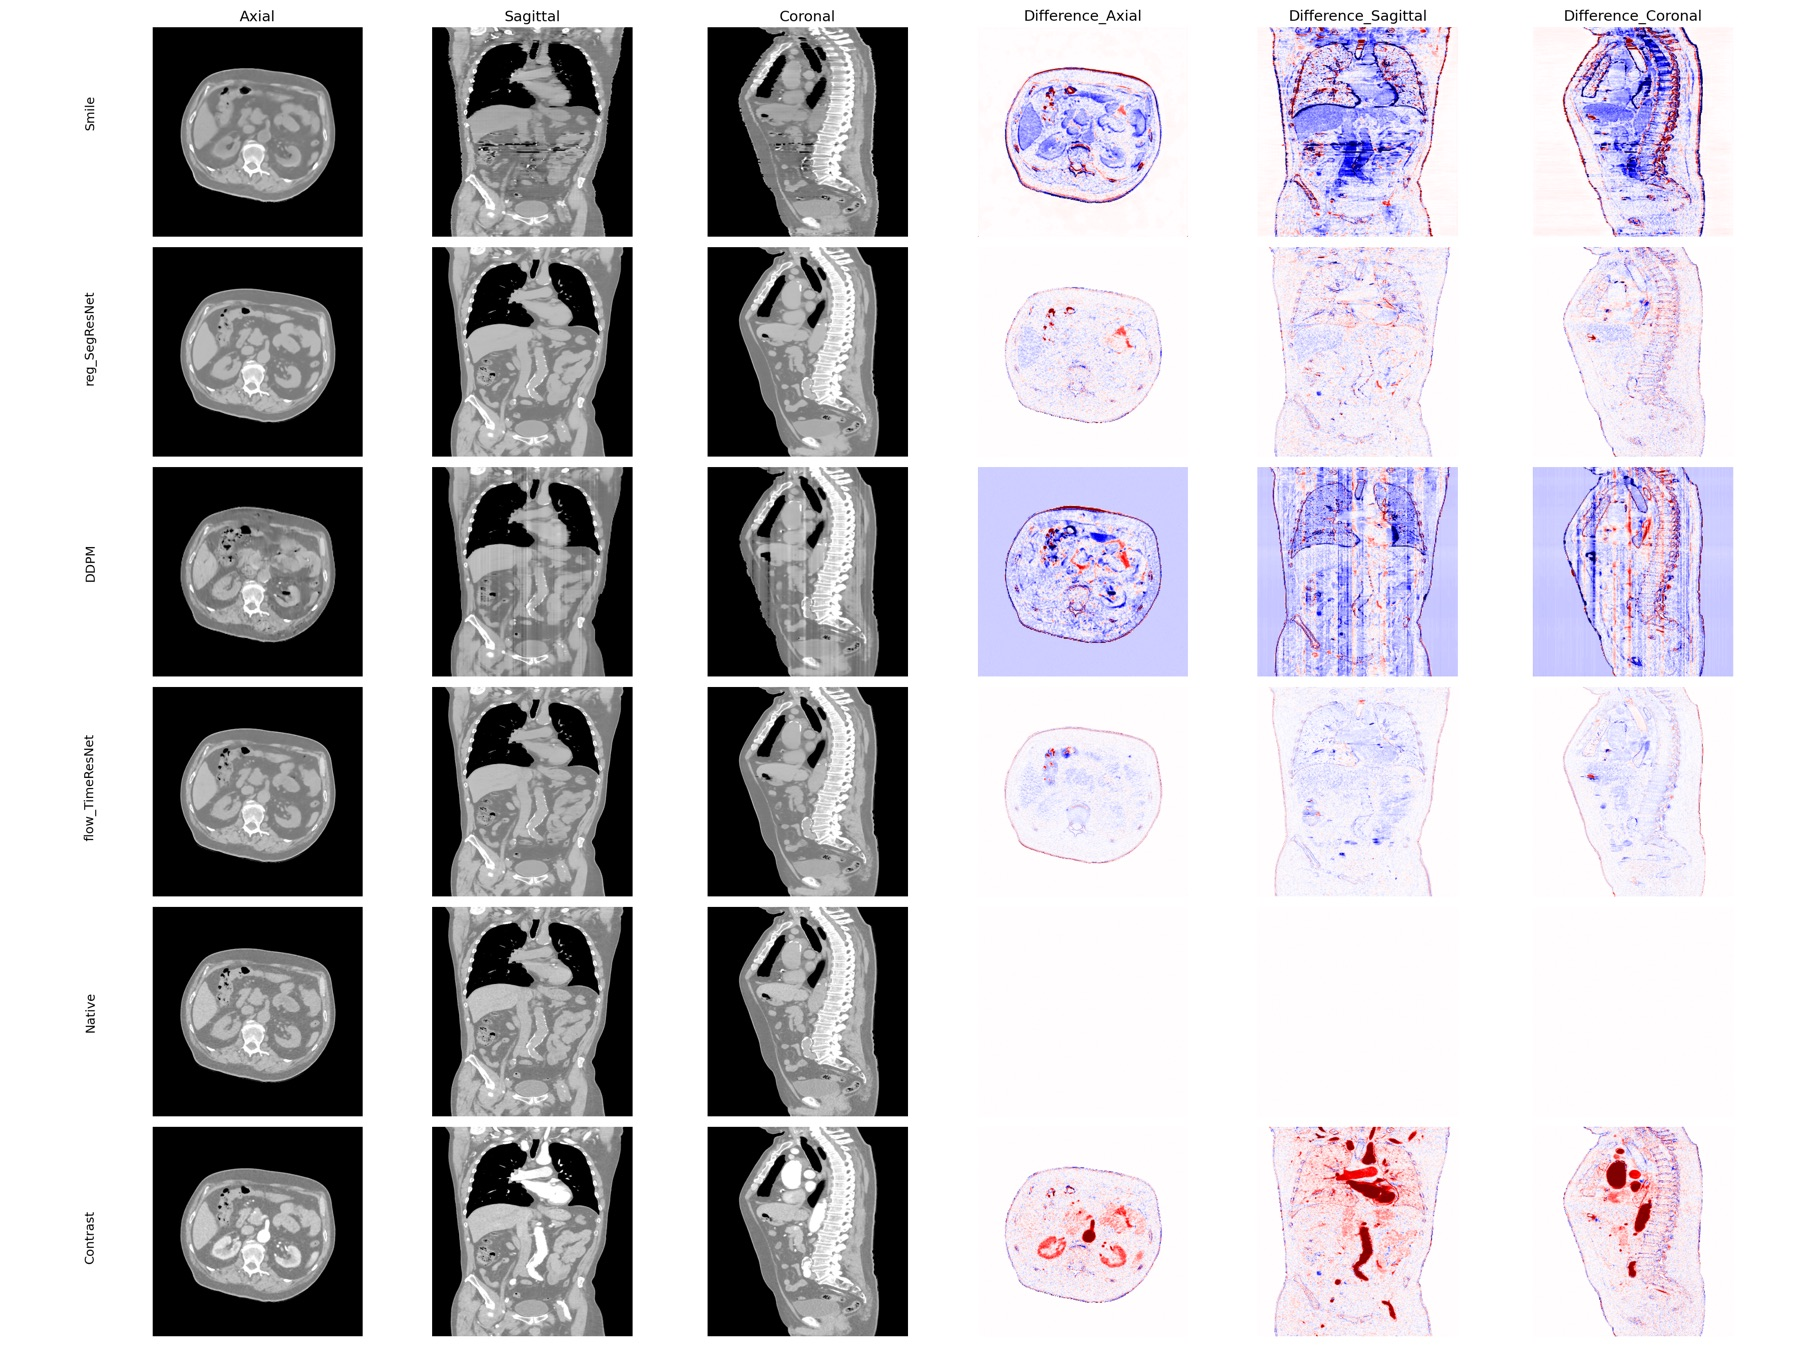
\includegraphics[width=\linewidth,height=0.70\textheight,keepaspectratio]{images/small_example.jpg}

\vspace{0.05cm}
{\scriptsize Аксиальный, сагиттальный, коронарный срезы + карты абсолютных ошибок.}
\end{column}
\begin{column}{0.44\textwidth}
\centering
{\scriptsize\textbf{Вклад компонент}}\\[0.08cm]
\renewcommand{\arraystretch}{0.95}
\resizebox{\linewidth}{!}{%
\begin{tabular}{lccc}
\toprule
\textbf{Вариант} & MAE$\downarrow$ & SSIM$\uparrow$ & PSNR$\uparrow$ \\
\midrule
TimeResNet & $\mathbf{4.25}$ & $\mathbf{.994}$ & $\mathbf{42.19}$ \\
\;без self-attn. & $5.96$ & $.985$ & $39.84$ \\
\;без time inj.  & $6.02$ & $.987$ & $39.96$ \\
\;без обоих      & $6.67$ & $.981$ & $38.52$ \\
\bottomrule
\end{tabular}}

\vspace{0.05cm}
{\scriptsize Удаление обоих ($+2.42$\,HU) $>$ суммы вкладов $\Rightarrow$ синергия.}

\vspace{0.25cm}
{\scriptsize\textbf{Downstream: nnUNet\,v2, аорта}}\\[0.08cm]
\renewcommand{\arraystretch}{0.95}
\resizebox{0.85\linewidth}{!}{%
\begin{tabular}{lc}
\toprule
\textbf{Обучение на} & \textbf{Dice}$\uparrow$ \\
\midrule
Реальные $\mathbf{x}_N$     & $0.966$ \\
Синтетические $\hat{\mathbf{x}}_N$ & $\mathbf{0.926}$ \\
\bottomrule
\end{tabular}}

\vspace{0.05cm}
{\scriptsize 95.9\% от уровня на реальных данных $\Rightarrow$ синтез пригоден для обучения сегментаторов.}
\end{column}
\end{columns}

\end{frame}

% ---- 13. Выносится на защиту ----------------------------------------
\begin{frame}{Выносится на защиту}
\small

\begin{enumerate}\setlength{\itemsep}{0.35em}
  \item \textbf{Medical Flow Matching} --- формализация трансляции КТ как переноса меры $\pi_N\leftrightarrow\pi_C$ с линейным интерполянтом и симуляционно-свободным обучением.

  \item \textbf{Двунаправленность}: $f_{\theta^*}=\argmin_f[\mathcal{L}^{N\to C}+\mathcal{L}^{C\to N}]$ --- одна сеть реализует оба направления без дообучения и без потери качества.

  \item \textbf{Одношаговый инференс}: постоянная целевая скорость линейного интерполянта позволяет интегрировать ОДУ за один шаг --- в $354\times$ быстрее DDPM без потери качества.

  \item Архитектура \textbf{TimeResNet} с двумя теоретически обоснованными компонентами: сохранение временного сигнала ($\partial\mathcal{L}/\partial t\neq0$) и боттлнек-внимание (сложность ниже в $4^{2k}$ раз).
\end{enumerate}

\begin{block}{Доклады и выступления}
Доклад на конференции МФТИ 2026; смежная работа подана на рецензируемый workshop CVPR 2026.
\end{block}


\end{frame}

\end{document}
